\documentclass[a4paper,14pt]{extreport} % формат документа

\usepackage{amsmath}
\usepackage{cmap} % поиск в ПДФ
\usepackage[T2A]{fontenc} % кодировка
\usepackage[utf8]{inputenc} % кодировка исходного текста
\usepackage[english,russian]{babel} % локализация и переносы
\usepackage[left = 2cm, right = 1cm, top = 2cm, bottom = 2 cm]{geometry} % поля
\usepackage{listings}
\usepackage{graphicx} % для вставки рисунков
\usepackage{amsmath}
\usepackage{float}
\usepackage{longtable}
\usepackage{multirow}
\graphicspath{{pictures/}}
\DeclareGraphicsExtensions{.pdf,.png,.jpg}
\newcommand{\anonsection}[1]{\section*{#1}\addcontentsline{toc}{section}{#1}}

\lstset{ %
	language=Prolog,                % Язык программирования 
	numbers=left,                   % С какой стороны нумеровать          
	frame=single,                    % Добавить рамку
}

\begin{document}
\begin{titlepage}

    \begin{table}[H]
        \centering
        \footnotesize
        \begin{tabular}{cc}
            \multirow{8}{*}{
\includegraphics[scale=0.35]{bmstu.jpg}}
            & \\
            & \\
            & \textbf{Министерство науки и высшего образования Российской Федерации} \\
            & \textbf{Федеральное государственное бюджетное образовательное учреждение} \\
            & \textbf{высшего образования} \\
            & \textbf{<<Московский государственный технический} \\
            & \textbf{университет имени Н.Э. Баумана>>} \\
            & \textbf{(МГТУ им. Н.Э. Баумана)} \\
        \end{tabular}
    \end{table}

    \vspace{-2.5cm}

    \begin{flushleft}
        \rule[-1cm]{\textwidth}{3pt}
        \rule{\textwidth}{1pt}
    \end{flushleft}

    \begin{flushleft}
        \small
        ФАКУЛЬТЕТ
        \underline{<<Информатика и системы управления>>\ \ \ \ \ \ \ 
        \ \ \ \ \ \ \ \ \ \ \ \ \ \ \ \ \ \ \ \ \ \ \ \ \ \ \ \ \ \ \ 
    \ \ \ \ \ \ \ \ \ \ \ \ \ \ \ } \\
        КАФЕДРА
        \underline{<<Программное обеспечение ЭВМ и
        информационные технологии>>
        \ \ \ \ \ \ \ \ \ \ \ \ \ \ \ \ \ \ \ \ }
    \end{flushleft}

    \vspace{4cm}

    \begin{center}
        \textbf{Лабораторная работа № 15} \\ 
        \hfill
        
        \textbf{Структура программы на Prolog и ее реализация} \\
        \vspace{0.5cm}
        \textbf{} \\
    \end{center}

    \vspace{4cm}

    \begin{flushleft}
        \begin{tabular}{ll}
            \textbf{Дисциплина} & Функциональное и логическое программирование \\
            \textbf{Студент} & Сиденко А.Г. \\
            \textbf{Группа} & ИУ7-63Б \\
            \textbf{Преподаватель} & Толпинская Н.Б., Строганов Ю.В.  \\
        \end{tabular}
    \end{flushleft}

    \vspace{4cm}

   \begin{center}
        Москва, 2020 г.
    \end{center}

\end{titlepage}

\textbf{Задание}

Создать базу знаний «Собственники», дополнив базу знаний, хранящую знания (лаб. 13):
\begin{itemize}
\item <<Телефонный справочник>>: Фамилия, №тел, Адрес – структура (Город, Улица, №дома, №кв),
\item <<Автомобили>>: Фамилия\_владельца, Марка, Цвет, Стоимость, и др.,
\item <<Вкладчики банков>>: Фамилия, Банк, счет, сумма, др.,
\end{itemize}
знаниями о дополнительной собственности владельца. Преобразовать знания об автомобиле к форме знаний о собственности.
Вид собственности (кроме автомобиля):
\begin{itemize}
\item Строение, стоимость и другие его характеристики;
\item Участок, стоимость и другие его характеристики;
\item Водный\_транспорт, стоимость и другие его характеристики.
\end{itemize}

Описать  и использовать вариантный домен: Собственность. Владелец может иметь, но только один объект каждого вида собственности (это касается и автомобиля), или не иметь некоторых видов собственности. 

\hfill

Используя конъюнктивное правило и разные формы задания одного вопроса, обеспечить возможность поиска:
\begin{enumerate}
\item Названий всех объектов собственности заданного субъекта,
\item Названий и стоимости всех объектов собственности заданного субъекта,
\item Разработать правило, позволяющее найти суммарную стоимость всех объектов собственности заданного субъекта.
\end{enumerate}

\hfill

Для 2-го пункт и одной фамилии составить таблицу, отражающую конкретный порядок работы системы, с объяснениями порядка работы и особенностей использования доменов (указать конкретные Т1 и Т2 и полную подстановку на каждом шаге)


\hfill

\textbf{Программа}

\begin{lstlisting}
domains
  lastname, city, street, model, color, bank, name = symbol
  telephone, house, flat, price, account, deposit, 
					     price = integer
  latitude, longitude = real
  adress = adress(city, street, house, flat)
  ownership = house(adress, price);
              ground(latitude, longitude, price);
	      auto(model, color, price);
	      boat(name, price)
        
predicates
  abonent(lastname, telephone, adress).
  depositor(lastname, city, bank, account, deposit).
  own(lastname, city, ownership).
  owns(lastname, city, name).
  ownsPrice(lastname, city, name, price).
  ownsSumPrice(lastname, city, price).
  boatPrice(lastname, city, price).
  housePrice(lastname, city, price).
  groundPrice(lastname, city, price).
  autoPrice(lastname, city, price).

clauses
  abonent(ellen, 111111, adress(moscow, tverskaya, 1, 1)).
  abonent(john, 222222, adress(moscow, arbat, 11, 112)).
  abonent(tom, 333333, adress(moscow, presnya, 10, 11)).
  abonent(eric, 444444, adress(moscow, pokrovka, 21, 55)).
  abonent(mark, 555555, adress(moscow, solyanka, 13, 13)).
  abonent(mark, 888888, adress(kazan, pushkin, 22, 130)).
  abonent(bill, 666666, adress(ekb, lenin, 12, 88)).
  abonent(bill, 777777, adress(spb, sadovaya, 1, 12)).
  depositor(ellen, moscow, sberbank, 10000, 2000).
  depositor(john, moscow, sberbank, 10000, 3000).
  depositor(john, moscow, vtb, 20000, 5000).
  depositor(tom, moscow, gazprom, 5000, 3000).
  depositor(eric, moscow, sberbank, 100000, 30000).
  depositor(mark, moscow, sberbank, 10000, 2000).
  depositor(mark, kazan, vtb, 10000, 2000).
  depositor(mark, moscow, gazprom, 10000, 2000).
  own(ellen, moscow, auto(bmw, red, 10000)).
  own(ellen, moscow, house(adress(moscow, tverskaya, 1, 1), 
					    	     100000)).
  own(tom, moscow, auto(mersedes, white, 15000)).
  own(tom, moscow, ground(48.40338, 52.17403, 50000)).
  own(eric, moscow, auto(mersedes, white, 20000)).
  own(eric, moscow, house(adress(moscow, pokrovka, 21, 55), 
					       	     200000)).
  own(eric, moscow, ground(28.40338, 32.17403, 500000)).
  own(eric, moscow, boat(ericary, 500000)).
  own(mark, moscow, auto(hyundai, silver, 7000)).
  own(mark, moscow, ground(41.40338, 2.17403, 100000)).
  own(mark, moscow, boat(mercury, 5000)).
  own(bill, ekb, auto(hyundai, black, 10000)).
  own(bill, ekb, house(adress(ekb, lenin, 12, 88), 50000)).
  own(bill, spb, auto(volvo, black, 13000)).
  own(bill, spb, house(adress(spb, sadovaya, 1, 12), 100000)).
  
  % Task1
  owns(Name, City, Types) :-
    own(Name, City, house(_, _)), Types = house.
  owns(Name, City, Types) :-
    own(Name, City, auto(_, _, _)), Types = auto.
  owns(Name, City, Types) :-
    own(Name, City, ground(_, _ ,_)), Types = ground.
  owns(Name, City, Types) :-
    own(Name, City, boat(_, _)), Types = boat.
  
  % Task2
  ownsPrice(Name, City, Types, Prices) :-
    own(Name, City, house(_, Prices)), Types = house.
  ownsPrice(Name, City, Types, Prices) :-
    own(Name, City, auto(_ ,_, Prices)), Types = auto.
  ownsPrice(Name, City, Types, Prices) :-
    own(Name, City, ground(_, _, Prices)), Types = ground.
  ownsPrice(Name, City, Types, Prices) :-
    own(Name, City, boat(_, Prices)), Types = boat.
  
  % Task3  
  housePrice(Name, City, Prices) :- 
    own(Name, City, house(_, Prices)),!.
  housePrice(_, _, Prices) :- 
    Prices = 0.
    
  groundPrice(Name, City, Prices) :- 
    own(Name, City, ground(_, _, Prices)),!.
  groundPrice(_, _, Prices) :- 
    Prices = 0.
    
  autoPrice(Name, City, Prices) :- 
    own(Name, City, auto(_ ,_, Prices)),!.
  autoPrice(_, _, Prices) :- 
    Prices = 0.
  
  boatPrice(Name, City, Prices) :- 
    own(Name, City, boat(_, Prices)),!.
  boatPrice(_, _, Prices) :- 
    Prices = 0.
      
  ownsSumPrice(Name, City, Prices) :-
    housePrice(Name, City, A),
    groundPrice(Name, City, B),
    autoPrice(Name, City, C),
    boatPrice(Name, City, D),
    Prices = A + B + C + D,
    Prices > 0.
\end{lstlisting}

\textbf{Примеры работы:}
\begin{enumerate}
\item Названий всех объектов собственности заданного субъекта,

\begin{lstlisting}
goal
  Name = eric,
  City = moscow,
  owns(Name, City, Types).
\end{lstlisting}


\includegraphics[scale=0.8]{ex1}

\item Названий и стоимости всех объектов собственности заданного субъекта,

\begin{lstlisting}
goal
  Name = bill,
  City = spb,
  ownsPrice(Name, City, Types, Price).
\end{lstlisting}

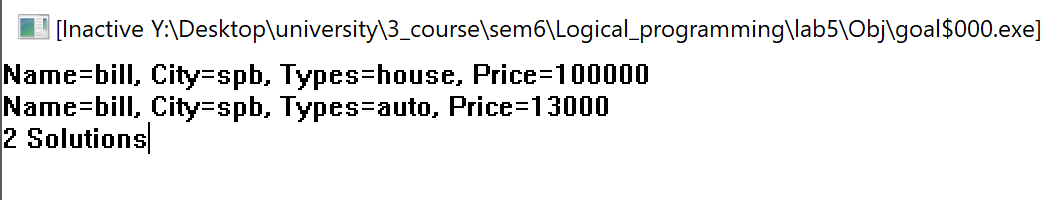
\includegraphics[scale=0.8]{ex2}

\item Разработать правило, позволяющее найти суммарную стоимость всех объектов собственности заданного субъекта.

\begin{lstlisting}
goal
  Name = bill,
  City = spb,
  ownsSumPrice(Name, City, Price).
\end{lstlisting}

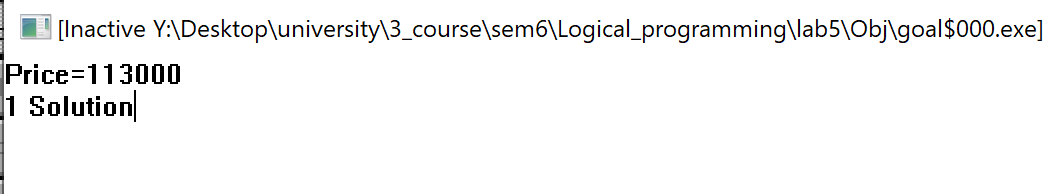
\includegraphics[scale=0.8]{ex3}

\end{enumerate}

\textbf{Приведем таблицу для задания 2. }

\begin{longtable}{|p{1.1cm}|p{8.5cm}|p{7cm}|}
	\hline
 	№ шага & Сравниваемые термы; результат; подстановка, если есть  & Дальнейшие действия: прямой ход или откат \\ \hline
	1 & По ownsPrice(Name, City, Types, Price)= ownsPrice(bill, spb, Types, Price) ищется системой определение отношения (по имени предиката и списку (числу) аргументов) & Определение отношения найдено, заносится в стек ownsPrice(bill, spb, Types, Price), прямой ход \\ \hline
	2 & Начинает <<раскрываться>> правило, т.е. доказывается каждое целевое утверждение в теле правила последовательно слева направо
	own(Name, City, house(\_, Prices)), Types = house.
	
	& Заносится в стек own(bill, spb, house(\_, Prices))\\ \hline

	3 & По own(bill, spb, house(\_, Prices))  ищется системой определение отношения (по имени предиката и списку (числу) аргументов) & Определение отношения найдено \\ \hline
	4 & Унификация own(bill, spb, house(\_, Prices)) с own(ellen, moscow, house(adress(moscow, tverskaya, 1, 1), 100000)) & Результат сравнения термов: false, переход к следующей строке (прямой ход) \\ \hline
	5 & Унификация own(bill, spb, house(\_, Prices)) с own(eric, moscow, house(adress(moscow, pokrovka, 21, 55), 200000)) & Результат сравнения термов: false, переход к следующей строке (прямой ход) \\ \hline
	6 & Унификация own(bill, spb, house(\_, Prices)) с own(bill, ekb, house(adress(ekb, lenin, 12, 88), 50000)) & Результат сравнения термов: false, переход к следующей строке (прямой ход) \\ \hline
	7 & Унификация own(bill, spb, house(\_, Prices)) с own(bill, spb, house(adress(spb, sadovaya, 1, 12), 100000)) & Результат сравнения термов: true, Prices примет значение 100000. Установим маркер. Анонимные переменные не связываются со значением. Переход к следующему целевому утверждению в теле правила (прямой ход) \\ \hline
	8 & Следующее целевое утверждение Types = house.  & Types принимает значение house, вывод результата \\ \hline
	9 &  &  В базе знаний больше ни одного утверждения с заданным именем, возврат, достаем из стека own(bill, spb, house(\_, Prices)) \\ \hline
	
	10 & Переход к следующему правилу с заданным именем, начинает <<раскрываться>> правило, т.е. доказывается каждое целевое утверждение в теле правила последовательно слева направо
	own(Name, City, auto(\_ ,\_, Prices)), Types = auto
	
	& Заносится в стек own(bill, spb, auto(\_ ,\_, Prices))\\ \hline

	11 & По own(bill, spb, auto(\_, Prices))  ищется системой определение отношения (по имени предиката и списку (числу) аргументов) & Определение отношения найдено \\ \hline
	12 & Унификация own(bill, spb, auto(\_, Prices)) с own(ellen, moscow, auto(bmw, red, 10000)) & Результат сравнения термов: false, переход к следующей строке (прямой ход) \\ \hline
	13 & Унификация own(bill, spb, auto(\_, Prices)) с own(tom, moscow, auto(mersedes, white, 15000)) & Результат сравнения термов: false, переход к следующей строке (прямой ход) \\ \hline
	14 & Унификация own(bill, spb, auto(\_, Prices)) с own(eric, moscow, auto(mersedes, white, 20000)) & Результат сравнения термов: false, переход к следующей строке (прямой ход) \\ \hline
	15 & Унификация own(bill, spb, auto(\_, Prices)) с own(mark, moscow, auto(hyundai, silver, 7000)) & Результат сравнения термов: false, переход к следующей строке (прямой ход) \\ \hline
	16 & Унификация own(bill, spb, auto(\_, Prices)) с own(bill, ekb, auto(hyundai, black, 10000)) & Результат сравнения термов: false, переход к следующей строке (прямой ход) \\ \hline
	17 & Унификация own(bill, spb, auto(\_, Prices)) с own(bill, spb, auto(volvo, black, 13000)) & Результат сравнения термов: true, Prices примет значение 13000. Установим маркер. Анонимные переменные не связываются со значением. Переход к следующему целевому утверждению в теле правила (прямой ход) \\ \hline
	18 & Следующее целевое утверждение Types = auto.  & Types принимает значение auto, вывод результата \\ \hline
	19 &  &  В базе знаний больше ни одного утверждения с заданным именем, возврат, достаем из стека own(bill, spb, auto(\_, Prices)) \\ \hline
	
	20 & Переход к следующему правилу с заданным именем, начинает <<раскрываться>> правило, т.е. доказывается каждое целевое утверждение в теле правила последовательно слева направо
	own(Name, City, ground(\_, \_, Prices)), Types = ground
	
	& Заносится в стек own(bill, spb, ground(\_ ,\_, Prices))\\ \hline

	21 & По own(bill, spb, ground(\_, Prices))  ищется системой определение отношения (по имени предиката и списку (числу) аргументов) & Определение отношения найдено \\ \hline
	22 & Унификация own(bill, spb, ground(\_, Prices)) с own(tom, moscow, ground(48.40338, 52.17403, 50000)) & Результат сравнения термов: false, переход к следующей строке (прямой ход) \\ \hline
	23 & Унификация own(bill, spb, ground(\_, Prices)) с own(eric, moscow, ground(28.40338, 32.17403, 500000)) & Результат сравнения термов: false, переход к следующей строке (прямой ход) \\ \hline
	24 & Унификация own(bill, spb, ground(\_, Prices)) с own(mark, moscow, ground(41.40338, 2.17403, 100000)) & Результат сравнения термов: false, в базе знаний больше ни одного утверждения с заданным именем, возврат, достаем из стека own(bill, spb, ground(\_, Prices)) \\ \hline

	25 & Переход к следующему правилу с заданным именем, начинает <<раскрываться>> правило, т.е. доказывается каждое целевое утверждение в теле правила последовательно слева направо
	own(Name, City, boat(\_, Prices)), Types = boat
	
	& Заносится в стек own(bill, spb, boat(\_ ,\_, Prices))\\ \hline

	26 & По own(bill, spb, boat(\_, Prices))  ищется системой определение отношения (по имени предиката и списку (числу) аргументов) & Определение отношения найдено \\ \hline
	27 & Унификация own(bill, spb, boat(\_, Prices)) с own(eric, moscow, boat(ericary, 500000)) & Результат сравнения термов: false, переход к следующей строке (прямой ход) \\ \hline
	28 & Унификация own(bill, spb, boat(\_, Prices)) с own(mark, moscow, boat(mercury, 5000)) & Результат сравнения термов: false, в базе знаний больше ни одного утверждения с заданным именем, возврат, достаем из стека own(bill, spb, boat(\_, Prices)) \\ \hline
	
	29 & Больше нет правил с заданным именем, достаем из стека ownsPrice(bill, spb, Types, Price) & Стек пуст, завершение программы \\ \hline
\end{longtable}

\hfill

\textbf{Ответы на вопросы}

\begin{enumerate} 
\item В какой части правила сформулировано знание? Это знание о чем, с формальной точки зрения?

Знания о предметной области выражаются на языке Пролог в виде предложений, называемых утверждениями (clauses). 

\item Что содержит тело правила?

Правило содержит несколько целей, которые должны быть истинными для того, чтобы правило было истинным.

<предикат>:–<предикат>[,<предикат>]*.

Символ <<:–>> означает «если». 
Символ <<,>> -- это логическая связка «и» или конъюнкция. 

\item Что дает использование переменных при формулировании знаний? В чем отличие формулировки знания с помощью термов с одинаковой арностью при использовании одной переменной и при использовании нескольких переменных? 

Предикат факта может содержать переменные в качестве аргументов. Такие факты называются универсальными: они истинны для любых значений переменных. 

Например,
любит(X, яблоко)

означает, что любой объект программы "любит яблоко". Универсальные факты сокращают запись программы.

Термы не содержащие переменных называются базовыми термами. Каждый такой терм именует вполне определенный объект. Если же терм содержит переменные, то он выступает в качестве представителя целого класса объектов, получающихся при подстановке различных термов вместо переменных.

\item С каким квантором переменные входят в правило, в каких пределах переменная уникальна? 

На все переменные в имени предиката наложен квантор всеобщности $\forall$, на переменные в теле предиката, которые отсутствуют в имени, наложен квантор существования $\exists$.

Областью действия переменной в Прологе является одно предложение. В разных предложениях может использоваться одно имя переменной для обозначения разных объектов. Исключением является анонимная переменная. Каждая анонимная переменная -- это отдельный объект.

\item Какова семантика (смысл) предложений раздела DOMAINS?  Когда, где и с какой целью используется это описание?

Домены должны быть определены до их использования. 

Раздел описания доменов является аналогом раздела описания типов в императивных языках программирования. 

Удобно использовать описание доменов для сокращения имен стандартных доменов. 

Например: i=integer
и далее использовать вместо ключевого слова integer односимвольное обозначение i.

Из доменов можно конструировать составные или структурные домены (структуры). 

Структура описывается следующим образом:

<имя структуры>=<имя функтора>(<имя домена первой компоненты>, ... , <имя домена последней компоненты>). 

\item Какова семантика (смысл) предложений раздела PREDICATES? Когда, и где используется это описание? С какой целью?

Предикаты должны быть определены до их использования. 

В разделе, озаглавленном зарезервированным словом PREDICATES, содержатся описания определяемых пользователем предикатов. В императивных языках программирования подобными разделами являются разделы описания заголовков процедур и функций. 

Описание n-местного предиката имеет следующий вид:

<имя предиката>(<имя домена первого аргумента>, ... , <имя домена n-го аргумента>).

Домены аргументов должны быть либо стандартными, либо объявленными в разделе описания доменов. 

Один предикат может иметь несколько описаний. 

\item Унификация каких термов запускается на самом первом шаге работы системы? Каковы назначение и результат использования алгоритма унификации? 

Пролог берет вопрос и начинает последовательно сверху-вниз сравнивать его с фактами и правилами базы знаний. То есть самыми первыми термами для унификации будет вопрос и первый факт/правило. 

Унификация двух термов -- это основной шаг доказательства. В процессе работы система выполняет большое число унификаций.
\textbf{Унификация} -- операция, которая позволяет формализовать процесс логического вывода. 

Унификация представляет собой процесс сопоставления цели с фактами и правилами базы знаний. Цель может быть согласована, если она может быть сопоставлена с заголовком какого-либо предложения базы.

\item В каком случае запускается механизм отката?

Откат дает возможность получить много решений в одном вопросе к программе. 

Во всех точках программы, где существуют альтернативы, в стек заносятся точки возврата. 

Если впоследствии окажется, что выбранный вариант не приводит к успеху, то осуществляется откат к последней из имеющихся в стеке точек программы, где был выбран один из альтернативных вариантов. 

Выбирается очередной вариант, программа продолжает свою работу. Если все варианты в точке уже были использованы, то регистрируется неудачное завершение и осуществляется переход на предыдущую точку возврата, если такая есть. 

При откате все связанные переменные, которые были означены после этой точки, опять освобождаются.

 \end{enumerate}
 
\end{document}